\documentclass[11pt]{article}
\usepackage[utf8]{inputenc}
\usepackage{amssymb, amsmath, amsthm, changepage, graphicx, caption, subcaption}

\graphicspath{{./images/}}

\title{MAT157 Problem Set 10}
\author{Nicolas}

\newcommand{\R}{\mathbb{R}}

\newcommand{\N}{\mathbb{N}}

\newcommand{\Z}{\mathbb{Z}}

\newcommand{\F}{\mathbb{F}}

\newcommand{\C}{\mathbb{C}}

\newcommand{\Q}{\mathbb{Q}}

\newenvironment{myproof}
{\begin{proof} \begin{adjustwidth}{3em}{0pt}$ $\par\nobreak\ignorespaces}
{\end{adjustwidth} \end{proof}} 

\begin{document}

\maketitle
\begin{flushleft}

1


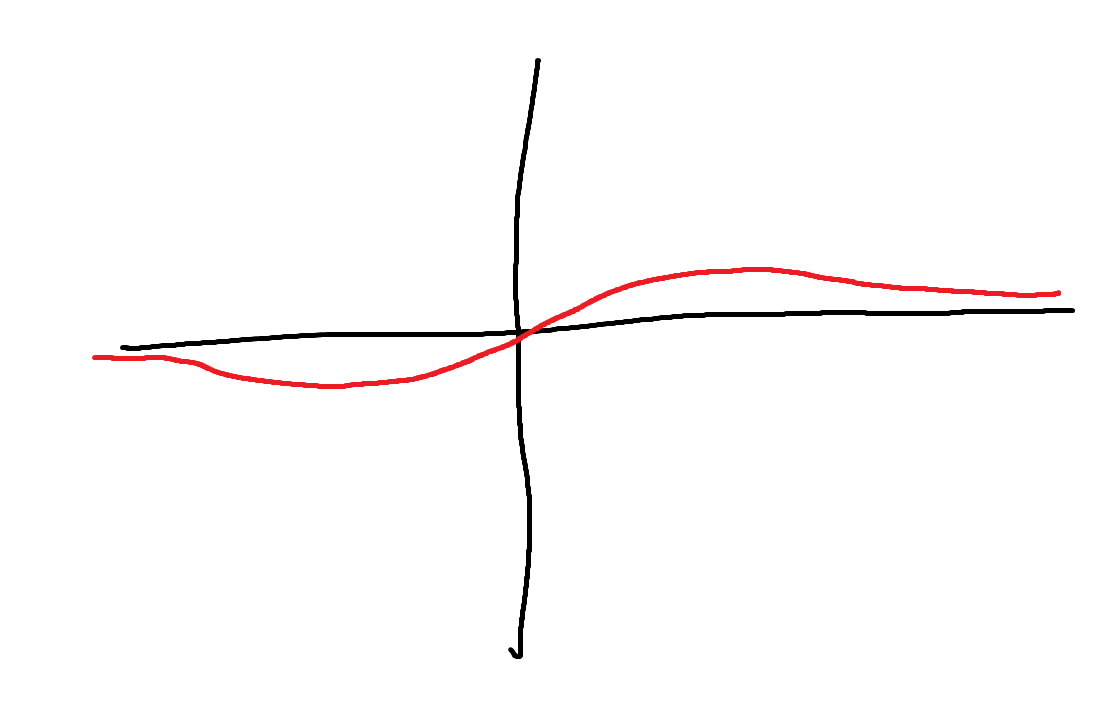
\includegraphics[width=\textwidth]{shittygraph.png}

\begin{align*}
&f:\R \to \R, \ f(x) = \frac{x}{1+x^2} \\
&f': \R \to \R, \ f'(x) = \frac{-(x^2-1)}{(x^2+1)^2} \\
&f'': \R \to \R, \ f''(x) = \frac{2x(x^2-3)}{(x^2+1)^2} \\
&f(0) = 0, \text{ so $f$ has a root at $x = 0$} \\
&f'(1) = f'(-1) = 0, \text{ so $f'$ has roots at $x = 1$ and $x = -1$} \\
&\text{This means that $f$ is incresing on the interval $(-1,1)$ because f' is positive on that interval.} \\
&\text{This means that $f$ is decreasing on the set $(-\infty, -1) \cup(1, \infty)$ because f' is negative on that set.} \\
& \text{We also may conclude that $f(1)$ is a local/global maxima, whereas $f(-1)$ is a local/global minima.} \\
&f''(0) = f''(\sqrt{3}) = f''(-\sqrt{3}) = 0, \text{ so $f''$ has roots at $x = 0, \sqrt{3}$ and $-\sqrt{3}$}. \\
&\text{This means that $f$ is concave up on the set $(-1,0)\cup(1, \infty)$ because $f''$ is positive on that set.} \\
&\text{This means that $f$ is concave down on the set $(-\infty, -1) \cup (0,1)$ because $f''$ is negative on that set.} \\
& \lim_{x \to \infty} f(x) = \lim _{x \to -\infty} f(x) = 0 \\
\end{align*}

\begin{myproof}

Let $\varepsilon > 0$ Choose $n > \frac{1}{\varepsilon}$. Then for every $x > n$, $|f(x)| = \frac{x}{1+x^2} < \frac{n}{1+n^2} < \frac{n}{n^2} = \frac{1}{n} < \varepsilon$ as desired. The proof is similar for $x \to -\infty$.

\end{myproof}

\newpage

2. a)

\begin{myproof}

Let $f:[a,b] \to \R$ and $P$ be an arbitrary partition of $[a,b]$. Let $[t_{i-1},t_i]$ be a interval induced by the partition $P$. If $f(x) \geq 0, \forall x \in [t_{i-1},t_i]$ then $f = |f|$, meaning $\sup f([t_{i-1},t_i]) - \inf f([t_{i-1},t_i]) = \sup |f|([t_{i-1},t_i]) - \inf |f|([t_{i-1},t_i])$. Now, consider $f(x) \leq 0, \forall x \in [t_{i-1},t_i]$ the $-f = |f|$, meaning $\sup f([t_{i-1},t_i]) - \inf f([t_{i-1},t_i]) = \sup |f|([t_{i-1},t_i]) - \inf |f|([t_{i-1},t_i])$ as well. If we consider our last alternative, $f(x)$ is neither all positive nor all negative (nor all zero, because that case is trivial) $\forall x \in [t_{i-1},t_i]$. Consider $M := \sup f([t_{i-1},t_i])>0$ and $m := \inf f([t_{i-1},t_i])<0$. Thus $M - m = M + |m|$. Now consider $M' := \sup |f|([t_{i-1},t_i])>0$ and $m' := \inf |f|([t_{i-1},t_i]) \geq 0$. Thus, $M' - m' \leq M' = \max \{ M, |m| \}$. Thus, $M'-m \leq \max \{ M, |m| \} < M - m$. Now, we have proven that for any arbitrary interval induced by the partition $P$ on $f$, $\sup |f|([t_{i-1},t_i]) - \inf |f|([t_{i-1},t_i]) \leq  \sup f([t_{i-1},t_i]) -  \inf f([t_{i-1},t_i])$. Thus, because this holds true for all intervals of any partitions, it simply follows that $U(|f|,P) - L(|f|,P) = \sum_{i = 0}^n M'_i (t_{i-1} - t_i) - \sum_{i = 0}^n m'_i (t_{i-1} - t_i) \leq \sum_{i = 0}^n M_i (t_{i-1} - t_i) - \sum_{i = 0}^n m_i (t_{i-1} - t_i) = U(f,P) - L(f,P)$ as desired.
\end{myproof}

b)

\begin{myproof}

It follows from part a) and \textit{Riemann's Criterion} that because $\forall \varepsilon > 0,U(|f|,P) - L(|f|,P) \leq U(f,P) - L(f,P) < \varepsilon$, then $|f|$ is also integrable.

\end{myproof}

c)

\begin{myproof}

Consider $f',g': \R \to \R, \ f'(x)= \frac{f(x)+|f(x)|}{2}, g'(x) = \frac{f(x)-|f(x)|}{2}$. We can very easily show that $f = f_+$ and that $g = f_-$. However, because $f_+$ is the sum of two integral functions ($f$ and $|f|$) and multiplication by a scalar $\frac12$, $f_+$ must also be integrable. It follows similarly for $f_-$.

\end{myproof}

d)

\begin{myproof}

Consider $f',g': \R \to \R, \ f'(x) := \frac{f(x)+g(x)+|f(x)-g(x)|}{2}, g'(x) := \frac{f(x)+g(x)-|f(x)-g(x)|}{2}$. It is easy to see that $\max = f'$ and $\min = g'$ (consider $x>y$ and vice-versa). Clearly, since $\max$ is sum of three integrable functions ($f,g$ and $|f-g|$) with a product of a scalar, $\max$ must be integrable. Similarly, $\min$ is also integrable.

\end{myproof}

\newpage

3.

\begin{myproof}

We will use induction on $n$. \\
Base Case: $n = 2$: $1^k \leq \frac{2^{k+1}}{k+1} \leq 1^k + 2^k$. As desired. \\
Induction Hypothesis: If $S_k(n-1) \leq \frac{n^{k+1}}{k+1} \leq S_k(n)$, then $S_k(n) \leq \frac{(n+1)^{k+1}}{k+1} \leq S_k(n+1)$. \\
Induction Step:
\begin{align*}
S_k(n) = &  \ S_k(n-1) + n^k \\
\leq & \ \frac{n^{k+1}}{k+1} + n^k \\
= & \ \frac{n^k(n+(k+1))}{k+1} \\
< & \ \frac{(n+1)^k(n+1)}{k+1} = \frac{(n+1)^{k+1}}{k+1}
\end{align*}

\end{myproof}

\newpage

4. a)

\begin{myproof}

Let $\varepsilon >0$ and consider any finite set of closed intervals $J_1,...,J_N$ such that $S \subseteq \bigcup_{i=1}^NJ_i, \ \sum_{i=1}^N(d_i - c_i)< \varepsilon', \ \varepsilon' \leq \min \{ \frac{\varepsilon}{b-a}, \frac{\varepsilon}{|\sup f([a,b]) - \inf f([a,b])|} \}$. Now, take a finite set of points $x_0,...,x_m$ such that the $\delta-$intervals (in respect to $\frac{\varepsilon'}{2}$) around each point is a finite cover of $[a,b]$. We will used the partition  $P := \{c_1,d_1,...,c_n,d_n \} \cup \{x_0,...,x_m \} \cup \{ a,b \}$. Thus, the distance between any two Riemann summands in the upper and lower Riemann sums is at most $\varepsilon'$. Thus, $U(f,P) - L(f,P) \leq \sum_{i=0}^{2n+m+3}\varepsilon' (t_i - t_{i-1})= \varepsilon' (b-a) < \varepsilon$. Because our choice of $\varepsilon$ was arbitrary, this allows us to use the \textit{Riemann Criterion} to prove that $f$ is integrable.

\end{myproof}

b)

\begin{myproof}

Let $\varepsilon > 0$ and consider any finite set of closed intervals $J_1,...,J_N$ such that $S \subseteq \bigcup_{i=1}^NJ_i, \ \sum_{i=1}^N(d_i - c_i)<  \varepsilon', \ \varepsilon' \leq \min \{ \frac{\varepsilon}{b-a}, \frac{\varepsilon}{\sup \{|f(x)-g(x)|: \forall x \in [a,b]\} } \}$. Now choose a partition $P$ of $[a,b]$ such that $U(f,P) - L(f,P) < \varepsilon'$. If we take the common refinement between $P$ and our set $\{ c_1,d_1,...c_n,d_n \}$ as our partition for $g$, $P'$ then we know that $U(f) - U(g,P') < \varepsilon' < \varepsilon$. Thus we can choose a partition that makes difference between the upper integral of $f$ and upper Riemann sum of $g$ in respect to $P'$ less than $\varepsilon$. We can do a similar thing to the lower integral of $f$ and the lower Riemann sum of $g$ in respect to $P'$. Since can make the difference between the upper and lower Riemann sums and $\int_{[a,b]}f$ less than $\varepsilon$, meaning we can choose a partition that makes $U(g,P)-L(g,P) < \varepsilon$, making it integrable following the \textit{Riemann Criterion}.
\\
\bigskip
The converse holds if we                                                                                                                                                                                                                                                                                                                                                                                                                                                                                                                                                                                                                                                                                                                                                                                                                                                                                                                                                                                                                                                                                                                                                                                                                                                                                                                                                                                                                                                                                                                                                                                                                                                                                                                                                                                                                                                                                                                                                                                                                                                                                                                                                                                                                                                                                                                                                                                                                                                                                                                                                                                                                                                                                                    just replace $f$ with $g$.

\end{myproof}

\newpage

5. a)

\begin{myproof}

We will first prove that $\sum_{k=0}^n {n \choose k}(-1)^{n-k}p(k) = \lambda n!$ for any polynomial of the form $p(x) = \lambda x^n$. We will induct on $n$. \\
Base Case: $n = 1$, $\sum_{k=0}^1 {n \choose k}(-1)^{1-k}p(k) = 0$ as desired. \\
Induction Hypothesis: If $\sum_{k=0}^n {n \choose k}(-1)^{n-k}p(k) = 0$, then $\sum_{k=0}^{n+1} {n+1 \choose k}(-1)^{n+1-k}p(k) = 0$. \\
Inductive Step: 
\begin{align*}
\sum_{k=0}^{n+1} {n+1 \choose k}(-1)^{n+1-k}p(k) = & \ \lambda (k-1)^{n+1} \\
= & \ \lambda (k-1)^n (k-1) \\
= & \ \sum_{k=0}^{n+1} {n \choose k}(-1)^{1-k}p(k) (k-1) \\
= & \ 0
\end{align*}

\end{myproof}



\end{flushleft}

\end{document}